\section{Ex. 1 - 2. Vandermonde matrix}
%\lstinputlisting{vandermonde.py}
In this section, we add the comments to the plots produced by the script given by: vandermonde.py .
For question (a), we are performing a polynomial interpolation on a set of data points using a 19th-degree polynomial, evaluated at $\approx$ 1000 equally-spaced points. The coefficients of the polynomial are determined by solving a system of linear equations using LU decomposition. We also plot the absolute difference between the given points $y_i$ and our result $y(x)$, i.e. $\abs(y(x) − y_i$. \\

From Fig.\ref{fig:lu_dec}, it seems that the polynomial is fitting the data points quite well for most of the range. This is expected as a polynomial of degree ($n$) can always fit ($n+1$) data points exactly. However, towards the end (around $x=100$), the polynomial shoots up drastically. This is a common issue with high-degree polynomial interpolation known as Runge's phenomenon. It is a form of overfitting where the polynomial oscillates significantly at the boundaries of the data set.

The choice of a 19th-degree polynomial for this data might not be the best. While it fits the given data points well, the extreme behavior at the boundaries suggests that it might not generalize well to other data. A lower-degree polynomial or a different type of function might provide a better fit without the extreme oscillations. \\

The bottom part of the plot shows the absolute difference between the given $y_i$ values and the calculated $y(x)$ values. This represents the error in the polynomial fit at the data points. Since the polynomial fits the data points exactly, these errors are close to zero, going from order $10^{-14}$ to $10^{-2}$. We can note how the error increases at the boundaries, consistently with the issue presented before. \\

For question (b), we implement Neville's algorithm and compare it to the results from LU decomposition (see Fig. \ref{fig:neville}).It works by recursively evaluating a set of polynomials and combining them to form the final interpolating polynomial. Regarding the interpolation, we are getting the same results, so they have same efficiency in fitting the given data points. The errors are drastically small for Neville's (reaching a maximum of $10^{-14}$) while LU decomposition have errors slightly higher. We could explain this addressing to the nature of the algorithm, which tends to be stable and accurate, especially when the data points are equally spaced. The accuracy of LU decomposition for interpolation can be influenced by the condition of the matrix involved. Ill-conditioned matrices may lead to numerical instability and higher errors. In our case, the condition number of the Vandermonde matrix depends on the arrangement and spacing of the data points. If the data points are well-spaced and not too close to each other, the condition number may be reasonable. However, as the data points become closely spaced or nearly collinear, the problem of ill-conditioning can arise. \\

For question (c) 




\begin{figure}[h!]
  \centering
  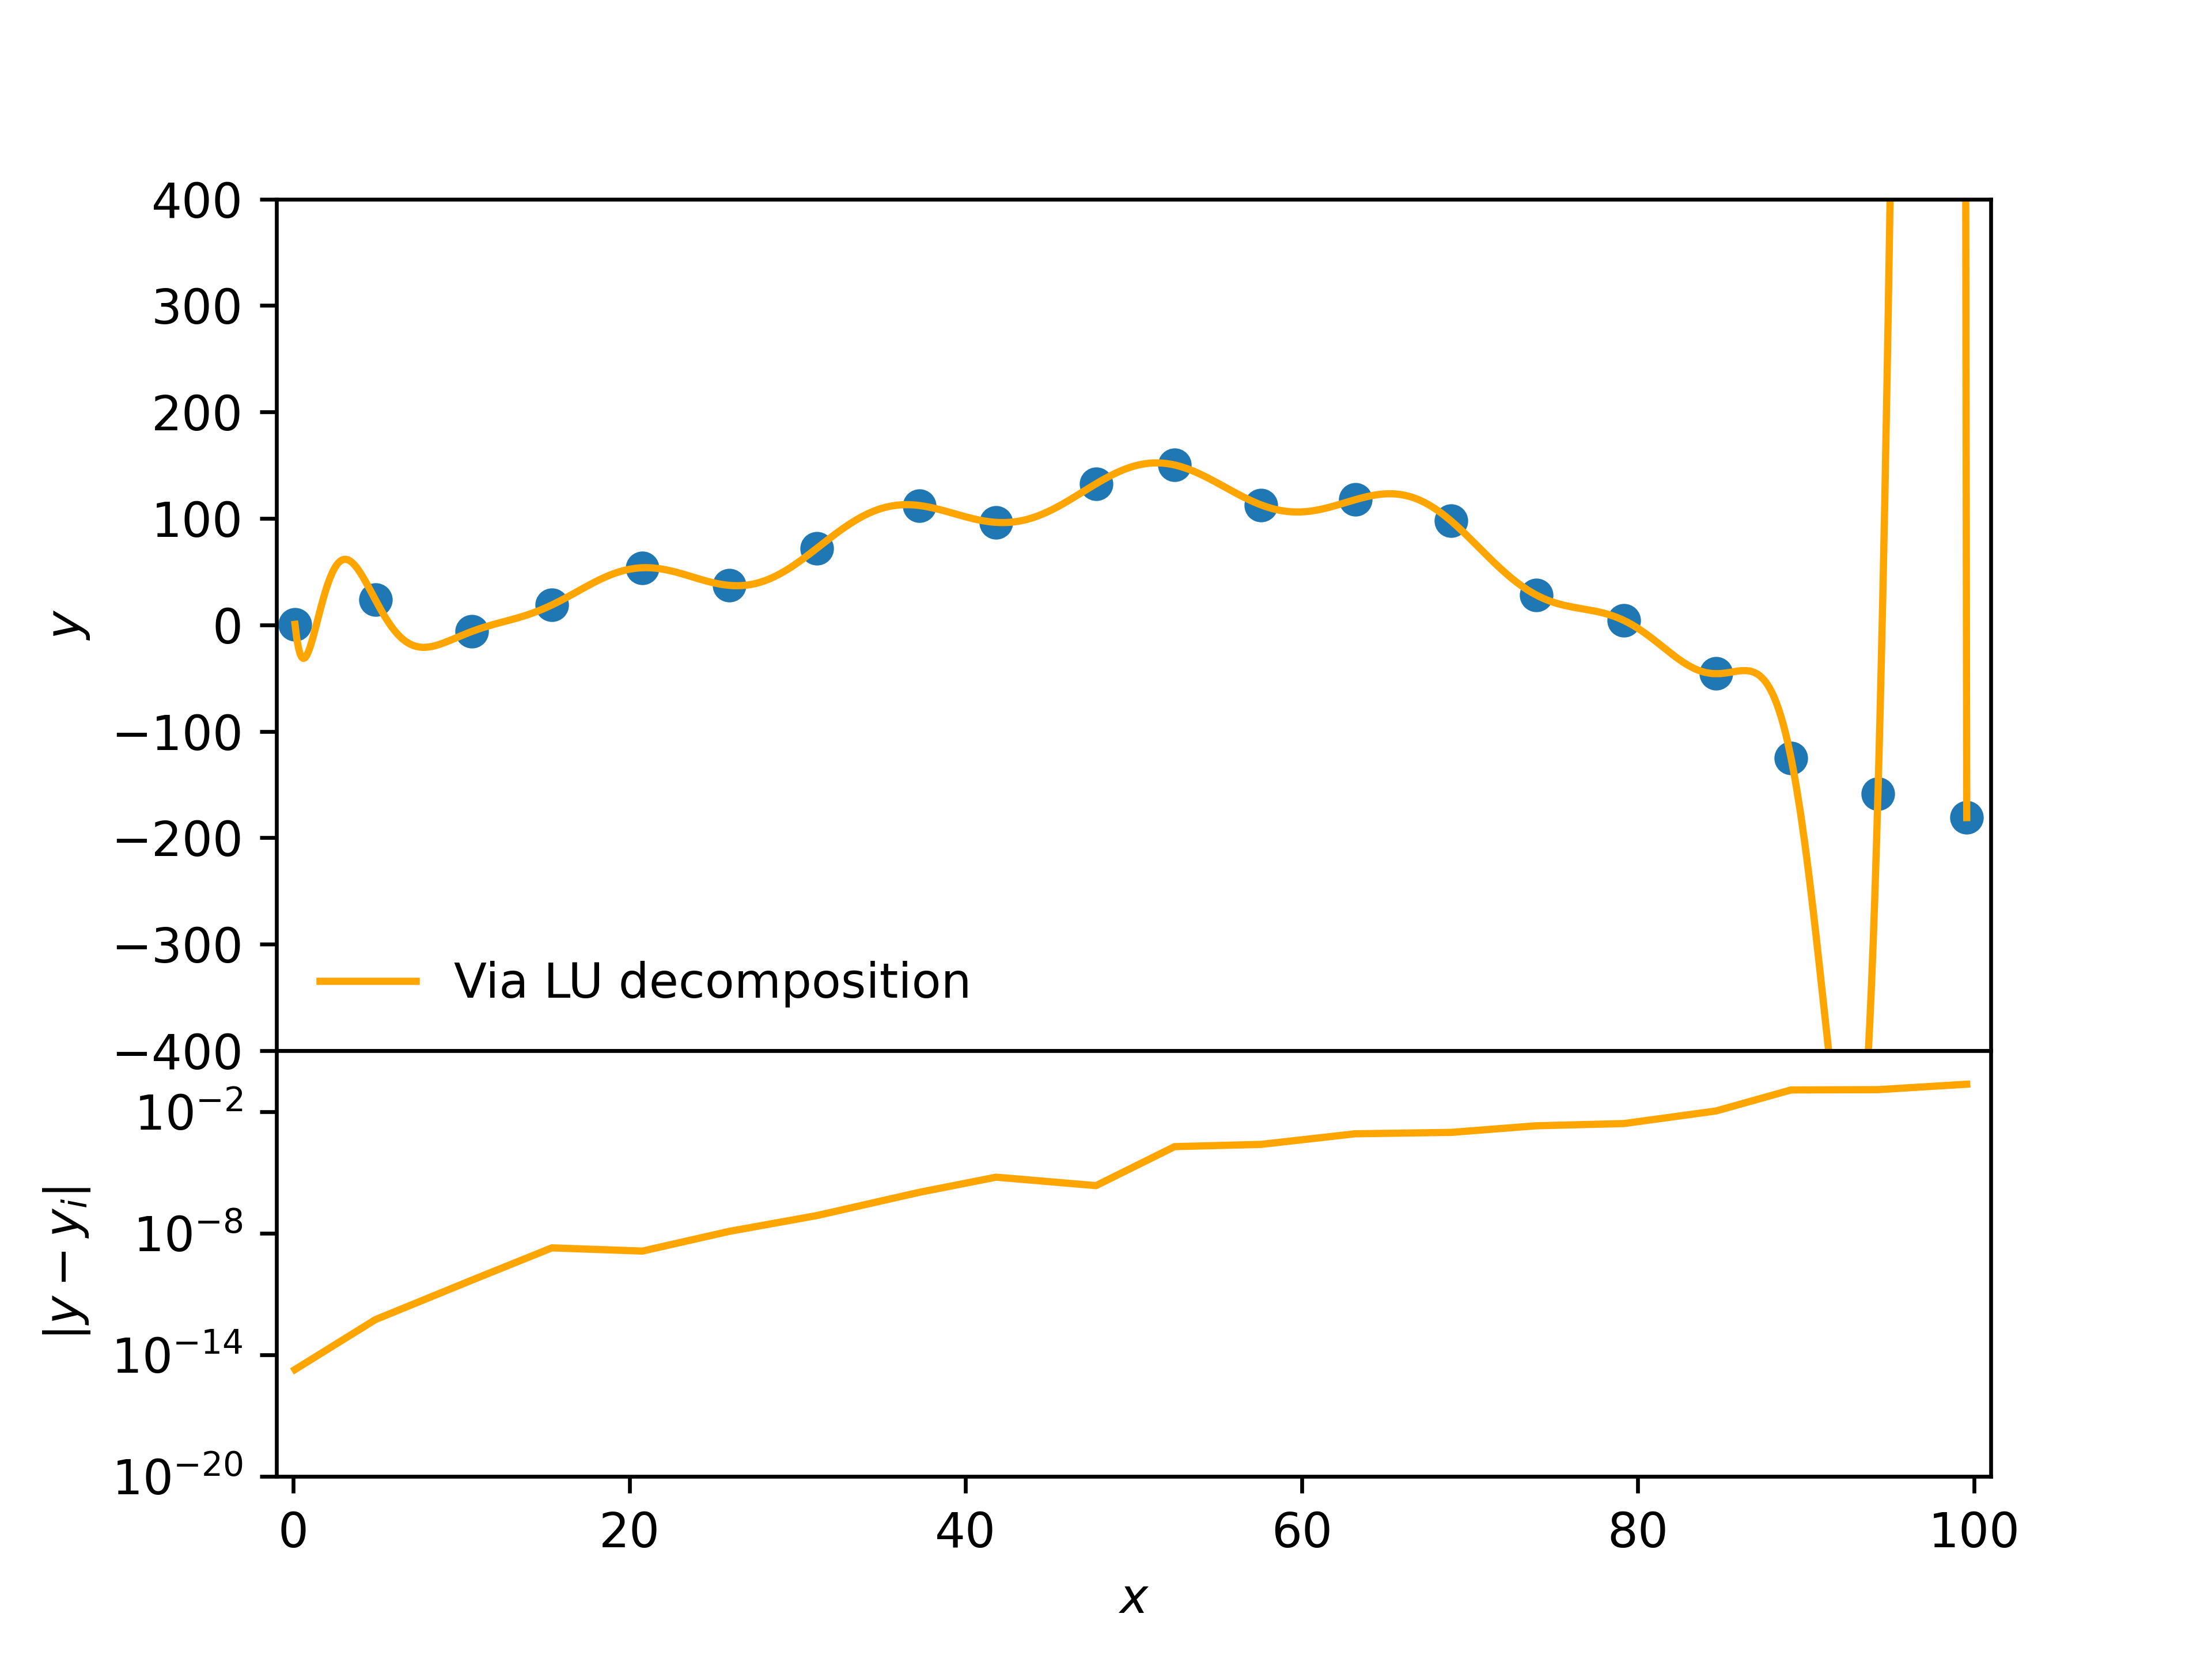
\includegraphics[width=0.9\linewidth]{.plots/my_vandermonde_sol_2a.png}
  \caption{Upper panel: Interpolation on a set of given data points via LU decomposition and Neville's. The fit is going through all the data points exactly. Nevertheless, it has an oscillating behaviour in correspondence of the last two points. Bottom panel: Absolute difference between the given points $y_i$ and our result $y(x)$, i.e. $\abs(y(x) − y_i$. The error holds at values close to zero, with a small increase towards the boundaries.}
  \label{fig:lu_dec}
\end{figure}

\begin{figure}[h!]
  \centering
  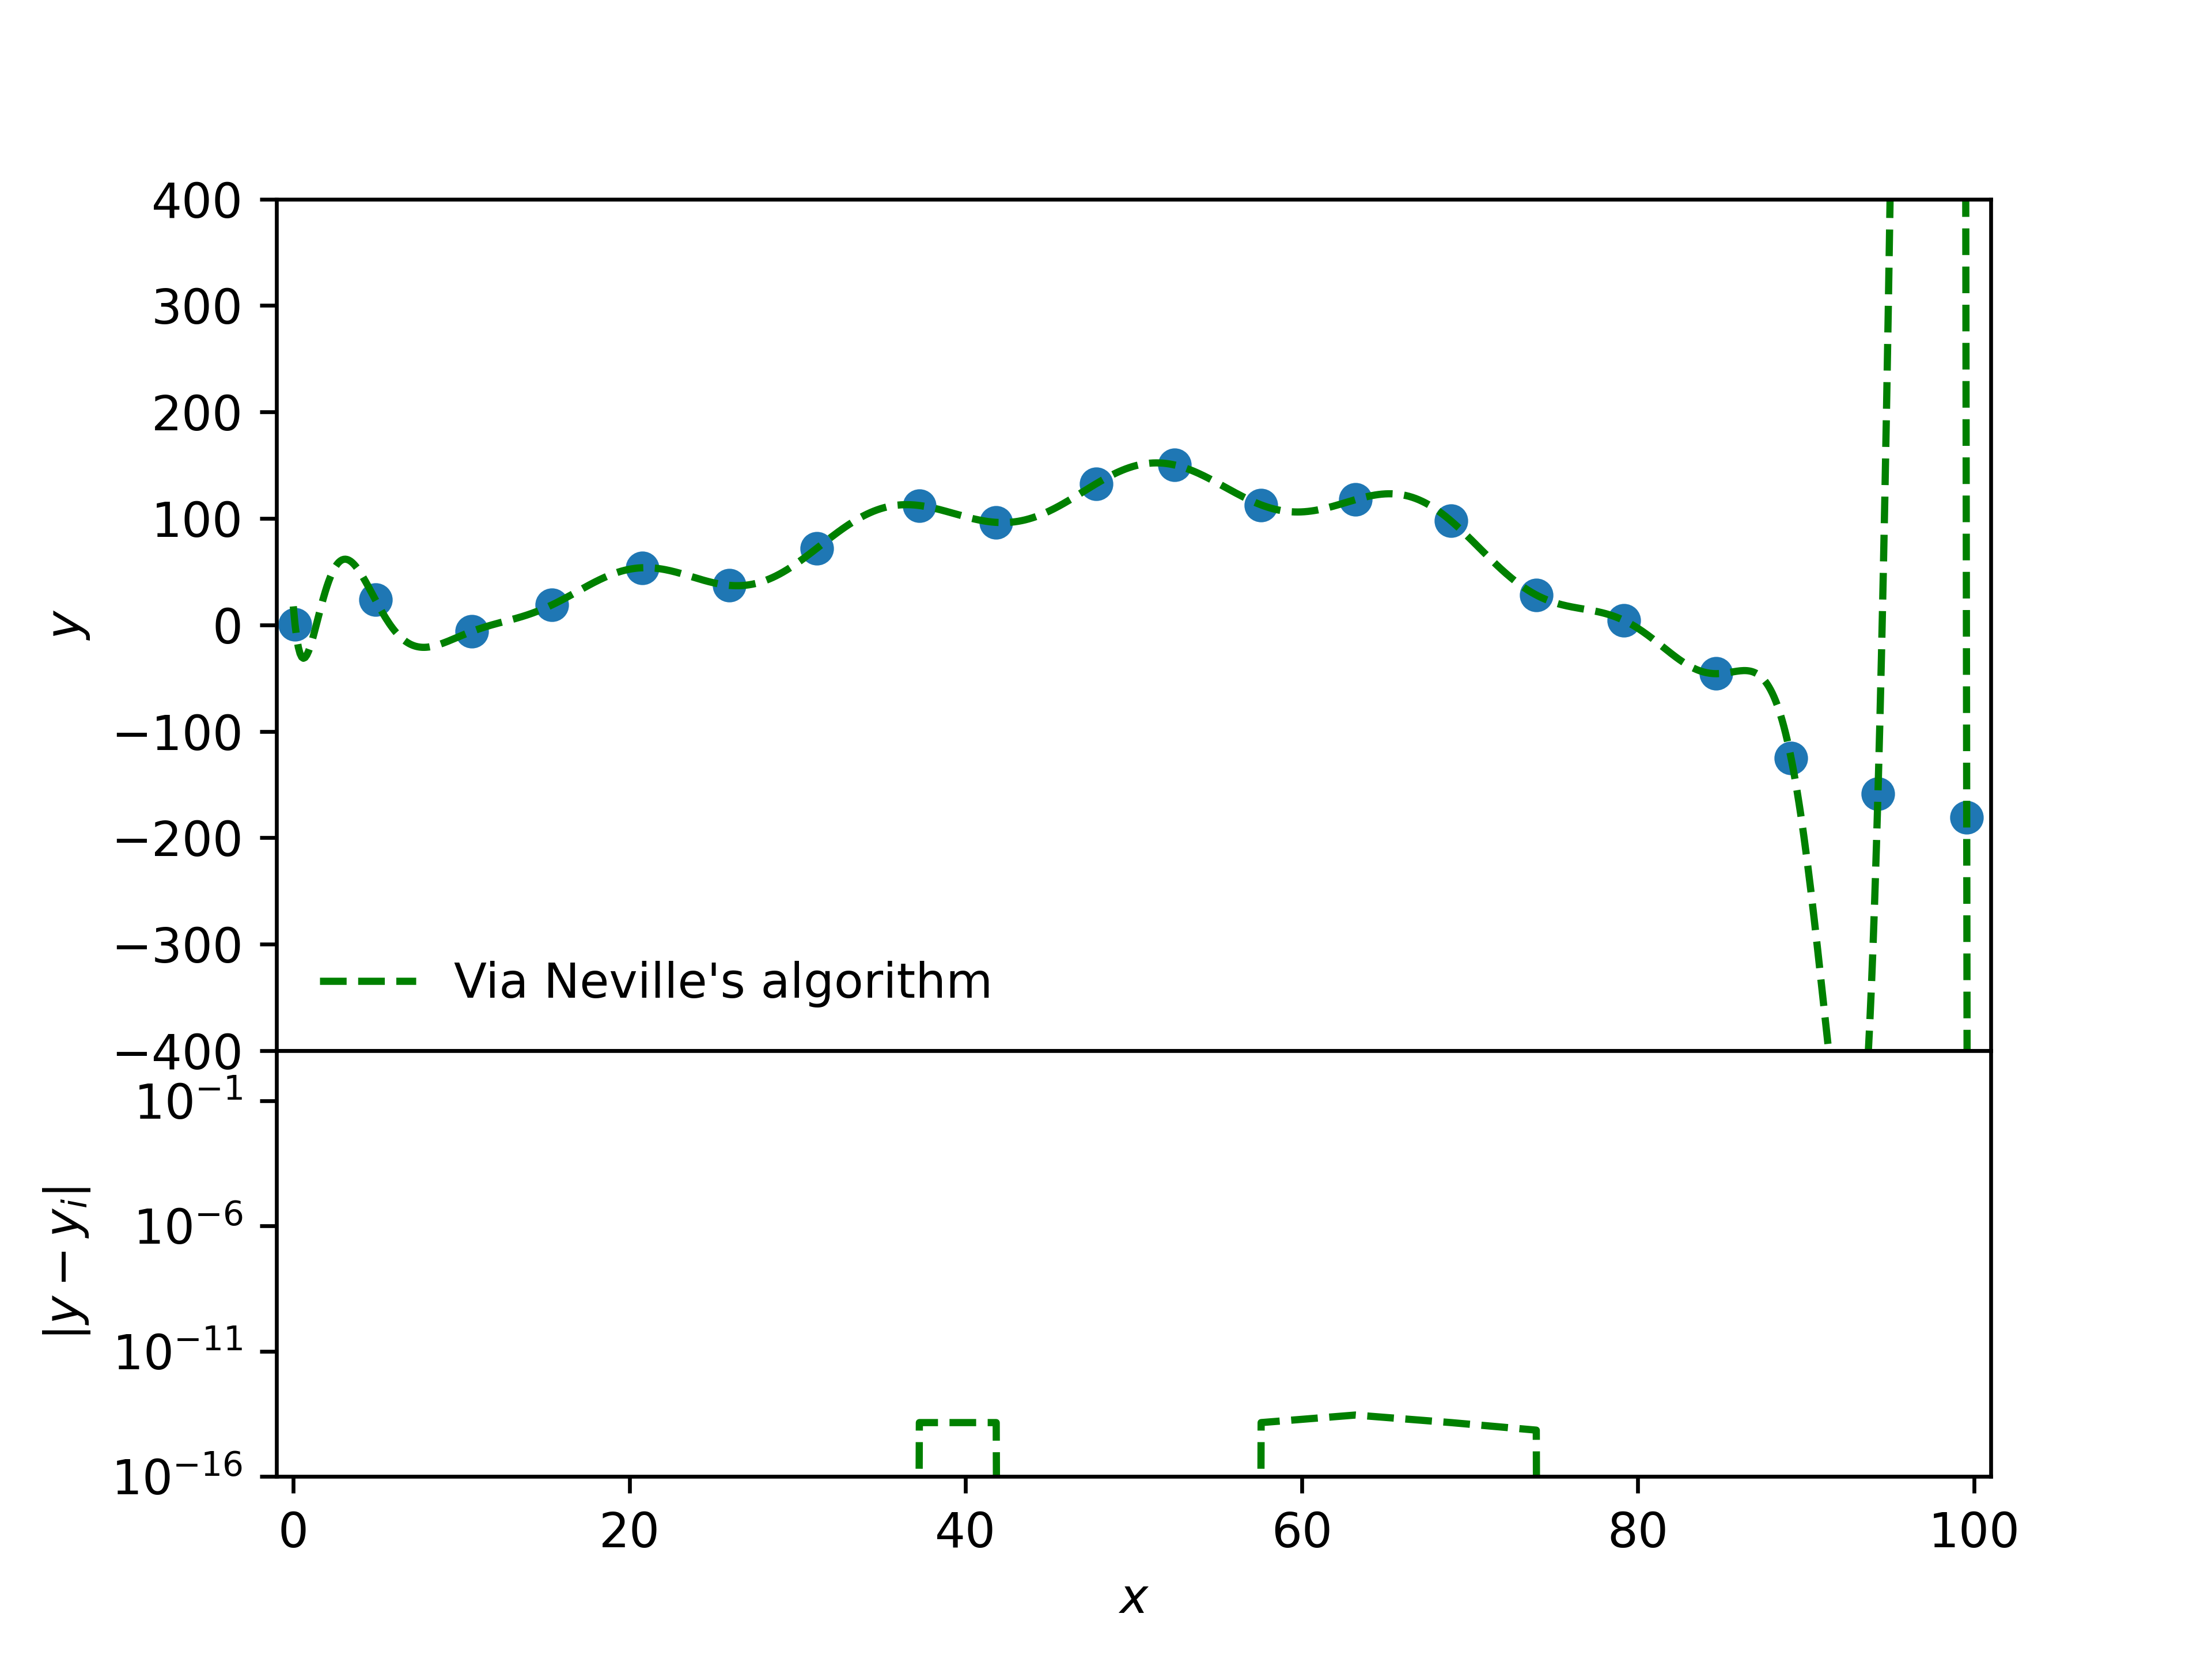
\includegraphics[width=0.9\linewidth]{.plots/my_vandermonde_sol_2b.png}
  \caption{Upper panel: Interpolation on a set of given data points via LU decomposition and Neville's algorithm. Both the polynomials obtained fits the data points well in the range considered, confirmed by their interpolations overlapping. Bottom panel: Absolute difference between the given points $y_i$ and our result $y(x)$, i.e. $\abs(y(x) − y_i$. The errors of Neville's algorithm reach very small values with respect to LU decomposition's ones. }
  \label{fig:neville}
\end{figure}
